\documentclass[12pt,twoside,a4paper]{article}

\renewcommand*\sfdefault{phv}
\renewcommand{\familydefault}{\sfdefault}

%\usepackage{arev}
\usepackage[scaled]{helvet}
\usepackage[T1]{fontenc}

%\newcommand{\Rapture}{${\mathbf{Rapture}}$~}
%\newcommand{\Reflex}{${\mathbf{Reflex}}$~}

\newcommand{\Rapture}{Rapture~}
\newcommand{\Reflex}{Reflex~}

\usepackage{listings}
\usepackage[usenames,dvipsnames,svgnames,table]{xcolor}
\usepackage{graphicx}
\usepackage{hyperref}
\usepackage{varioref}

\newcommand{\myTitle}{ RaptureAPI\xspace}
\newcommand{\myClient}{\xspace}
\newcommand{\myName}{Alan Moore\xspace}
\newcommand{\myTime}{February 12, 2016\xspace}
\newcommand{\myCFootnote}{Documentation By\xspace}
\newcommand{\myCompany}{Incapture\xspace}
\newcommand{\myCompanyFull}{Incapture Technologies LLC\xspace}
\newcommand{\myCompanyAddress}{600 Montgomery Street\\San Francisco \\ CA 94111\xspace}

\parskip 5pt

\makeindex

\lstdefinelanguage{reflex}
{
  morekeywords={def,end,for,while,if,else,do,const,println,fromjson,json},
  morecomment=[l]{//},
  morestring=[b]"
}

\definecolor{mygray}{rgb}{0.95,0.95,0.95}
\lstset{basicstyle=\footnotesize\ttfamily,breaklines=true}

\lstset{ %
  aboveskip=7pt,
  belowskip=7pt,
  numberbychapter=false,
  %language=reflex,                % the language of the code
  %basicstyle=\small,           % the size of the fonts that are used for the code
  numbers=left,                   % where to put the line-numbers
  backgroundcolor=\color{mygray},
  numberstyle=\tiny\color{gray},  % the style that is used for the line-numbers
  keywordstyle=\color{blue},
  stringstyle=\color{red},
  stepnumber=1,                   % the step between two line-numbers. If it's 1, each line
  numbersep=7pt,                  % how far the line-numbers are from the code
  columns=fixed,
  showspaces=false,               % show spaces adding particular underscores
  showstringspaces=false,         % underline spaces within strings
  showtabs=false,                 % show tabs within strings adding particular underscores
  frame=TB,                   % adds a frame around the code
  rulecolor=\color{black},        % if not set, the frame-color may be changed on line-breaks within not-black text (e.g. commens (green here))
  tabsize=2,                      % sets default tabsize to 2 spaces
  captionpos=b,                   % sets the caption-position to bottom
  breaklines=true,                % sets automatic line breaking
  breakatwhitespace=false,        % sets if automatic breaks should only happen at whitespace
  escapeinside={\%*}{*)},            % if you want to add LaTeX within your code
  morekeywords={*,...}               % if you want to add more keywords to the set
}

\begin{document}

\title{The Rapture API}
\author{Alan Moore}
\date{February 2016}

\maketitle
\tableofcontents

\section{Background}
\Rapture is a platform system that can be used to build applications that are scalable,
distributed, consistent and coordinated. At its heart \Rapture is simply a well defined
set of libraries with an external facing api that provides an abstraction to a number
of fundamental concepts. This document describes the APIs of \Rapture in detail from the
perspective of a programmer - alongside each API call are sections on their use within
\Rapture and typical use cases for that API or API set.

The general architecture of a \Rapture system is reproduced in Figure~\vref{fig:RaptureDiagram}.

\begin{figure}[htb]
\centering
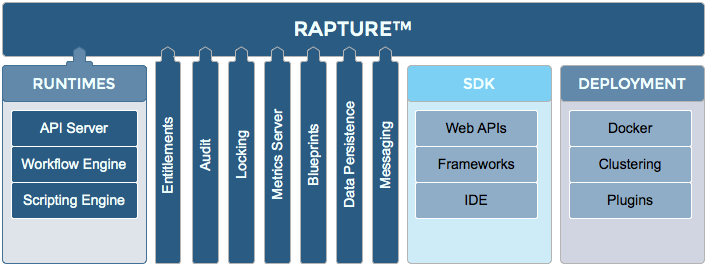
\includegraphics[width=15cm]{Graphics/rapturecore}
\caption{Rapture Component Parts}
\label{fig:RaptureDiagram}
\end{figure}

Applications that interact with \Rapture, or are \emph{hosted} on \Rapture will
use the \Rapture API to interact with this underlying framework. The goal of
the \Rapture API is that the interaction with \Rapture is invariant to the location
of the application -- the API looks \emph{the same} no matter where the application
resides.

\section{Application Locations}
Applications interacting with \Rapture will typicall fall within one of the
following categories.

\begin{itemize}
  \item{Client applications interacting with a remote \Rapture environment.}
  \item{Client \Reflex scripts using the ReflexRunner application.}
  \item{Server applications embedding the \Rapture kernel.}
  \item{Scripts running on a server that is itself running the \Rapture kernel.}
  \item{Extensions to \Reflex or repository or message drivers.}
  \item{Scripts run in the context of an ajax call from a web browser.}
\end{itemize}

\subsection{Context and Entitlements}
Every interaction with a \Rapture API call is made in the context of a logged in
user. That user, and its entitlement group membership and the parameters passed
to the call are used to determine whether the call can proceed or not. If an
API call is used to run a script on \Rapture or to start a workflow \emph{that} script
or workflow is run in the context of the calling user as well.

In some API use categories the interface used to interact with the \Rapture API
is already bound to a user - typically this is for processes that are running
server side. Client side use cases usually have to \emph{login} to \Rapture first,
providing credentials that get translated by the \Rapture API into a \verb+CallingContext+
value (a token) which can then be used in subsequent calls to identify the user
making the call. In some client side languages there are helper constructs that
can be used to automatically pass in the logged in context to the API calls,
leaving the programmer free to not worry about this aspect.

Wrapper applications such as ReflexRunner log in on the caller's behalf and then
pass that logged in API context to the underlying container that runs the script.

\subsection{Custom client applications}

Client applications that talk to \Rapture can be written in any of these supported languages as
long as the application can reach (using TCP/IP) a \Rapture API Server.

\begin{itemize}
  \item{Java (or anything that runs on the Java VM and can access Java classes.)}
  \item{.NET}
  \item{Python}
  \item{Javascript (typically node.js, see a later section on architectures for browser applications.)}
  \item{Ruby}
  \item{Go(lang)}
\end{itemize}

The transport between client and server uses a JSON-RPC style of communication which
means that other language support can easily be added. The build process for
\Rapture can autogenerate client side stubs once an initial template has been
created - the authors created the .NET implementation in a few hours.

Typically the use of \Rapture in these applications follows this pattern:

\begin{enumerate}
  \item{Obtain the ip address or name of the \Rapture environment API endpoint.}
  \item{Obtain the user name and password for the use of the API.}
  \item{Call a login function to obtain a calling context.}
  \item{Pass that login context into a wrapper (for future API use) or simply pass the context into future API calls.}
\end{enumerate}

For example in Java here is a simple code extract for the login and API use process:

\begin{lstlisting}[caption={Java simple example}, language=Java]
  String host = "test.incapture.net";
  String username = "test";
  String password = "secret";
  SimpleCredentialsProvider creds = new SimpleCredentialsProvider(username, password);
  HttpLoginApi loginApi = new HttpLoginApi(host, creds);
  loginApi.login();

  ScriptClient client = new ScriptClient(loginApi);
  String content = client.getDoc().getContent("//testRepo/doc/one");
  System.out.println(content);
\end{lstlisting}

This example logs into a \Rapture environment and passes that logged in context to a \verb+ScriptClient+
instance. It is this script client that can then be easily used to interact with \Rapture. The
\verb+getContent+ call in the document API will be described in detail later.

In Python, the equivalent interaction is reproduced below:

\begin{lstlisting}[caption={Python simple example}, language=Python]
  import raptureAPI
  url = 'test.incapture.net'
  username = 'test'
  password = 'secret'
  rapture = raptureAPI.raptureAPI(url, username, password)
  content = rapture.doDoc_GetContent('//testRepo/doc/one')
  print content
\end{lstlisting}

Here we see a similar login approach and then the invocation of the same \Rapture
API call. With the same target \Rapture environment these two code snippets will
produce exactly the same output.

\subsection{Client \Reflex scripts}

\Reflex scripts running on the client (or the server) are always running in a
container that has already been connected to an environment -- the wrapper is
the piece of code that has logged into \Rapture already.

In \Reflex then the code is even simpler. In fact \Reflex has some additional
syntax sugar for loading documents from \Rapture.

\begin{lstlisting}[caption={Reflex simple example}, language=reflex]
  contentAsMap <-- "//testRepo/doc/one";
  println(contentAsMap);

  // or

  content = #doc.getContent("//testRepo/doc/one");
  contentAsMap = fromjson(content);
  println(contentAsMap);
\end{lstlisting}

In the second access example we convert the raw JSON formatted document from
\Rapture into a \Reflex map structure so as to make the two approaches produce
the same output.

\subsection{Server side kernel applications}

If a Java (or Java VM) application embeds the \Rapture kernel code within it the
means for calling the \Rapture API can have a number of forms. Code running within
\Rapture has to be much more careful about calling contexts and who is actually
making the call, and there is no need to worry about host urls because the code
is running directly on \Rapture.

One approach to running the same example code is reproduced below:

\begin{lstlisting}[caption={Kernel simple example}, language=Java]
   CallingContext userContext = Kernel.getLogin().login(
          "test", "secret", null);
   String content = Kernel.getDoc().getContent(
          userContext, "//testRepo/doc/one");
   System.out.println(content);
\end{lstlisting}

Note that to run the above code your server application will have had to initialize
and configure itself first, something which is outside the scope of this document
but will trivially be a matter of defining configuration files for connection to
underlying data stores and then calling:

\begin{lstlisting}[caption={Kernel initialization}, language=Java]
   Kernel.initBootstrap();
\end{lstlisting}

\section{Application Location Summary}
Applications can sit in many places in the architecture of a solution that
includes a \Rapture system. The goal of the \Rapture API is to make the access
to \Rapture as simple and consistent as possible to all applications so it is
easy for a developer to move their applications within the system architecture or
to switch and change the programming languages used for an application.

\section{API Introduction}
The \Rapture API is divided into a number of sections. We've seen in an earlier
section how you may need to use the \emph{login} api to establish a connection
to \Rapture. The other sections of the API will form the rest of this document.
For each section the general positioning of the section with respect to \Rapture
will be described and then the detailed API calls will follow.

\section{Doc API}
Plugins in \Rapture are installable items that can be released to a \Rapture environment in
a consistent way. There are three parts to the Plugin API.

The first part relates to retrieving information about what is actually installed, and what items were installed with each
plugin. These are used by operator consoles and are informational.

The second part relates to installing an actual plugin. These calls are typically used by a specific
client side application "PluginInstaller" or a self installing library that uses the "SelfPluginInstallerLib". Plugins
defined in this way are jar archives that have a very specific structure. Typically a developer lays out this structure
in the file system and then uses a build process to package this information up into a jar file which can then be used with
the PluginInstaller application.

\section{File layout of a plugin}

A sample layout of a plugin "on disk" is reproduced below:

\begin{Verbatim}
  -- src/main/resources
     - PLUGIN
        - plugin.txt
        - content
          - testRepo
             - .rdoc
             someContent.rdoc
          - myscripts
             - test.script
\end{Verbatim}

The mandatory aspects of a plugin are the concept of a PLUGIN folder in the resources within
which is a plugin.txt file. This file has a specific format, an example is reproduced below:

\begin{Verbatim}
  {
     "depends":{},
     "description":"Curtis Web Core",
     "plugin":"CurtisWebCore",
     "version":{
     		"major":1,
     		"minor":1,
     		"release":32,
     		"timestamp":99999999999999
     }
  }
\end{Verbatim}

Most of these fields are self describing - the "plugin" field is the unique reference (uri) of this
plugin and the version section defines the version \emph{of this plugin}. The description is for operators
and the depends field can contain a map of other plugins and their version numbers required.

\section{Plugin file types}

The content folder contains information and definitions for content and configuration that this plugin defines. The
file name extension defines what the plugin installer will do for this item.

\begin{table}[H]
\begin{center}
\begin{tabular}{r p{10cm}}
  Extension & Purpose \\
  \hline
  script & Defines a \Reflex script. The full uri of the script is formed from this file's location in the content directory.\\
  series & Defines set of points in a series (if fully named) or the definition of a series repository. In the latter case the .series file
     must be at the 2nd top level folder in the content folder - the name of the folder is the name of the repository in \Rapture. \\
  blob & Defines a blob in a blob repository or the definition of a blob repository (if the file is .blob). Note that files that are not in
    the list of extensions in this table are treated as blobs, with the mime type inferred from the extension of the file. \\
  rdoc & Defines a document in a document repository \emph{or} the definition of a document repository (if no name specified). \\
  idgen & Defines an idgenerator. The name of the generator is defined by the top level folder, the contents is the configuration of an ID generator.\\
  revent & Defines a rapture event. The content of the file is a RaptureEvent structure (as json). \\
  table & Defines a rapture table. The name of the table is the enclosing folder. \\
  job & Defines a schedule job. \\
  workflow & Defines a workflow. \\
  lock & Defines a lock manager. \\
  structured & Defines a structure store reference. \\
\end{tabular}
\end{center}
\end{table}

In all cases for these files where the content drives the definition of something in \Rapture, the content is
a json formatted document that is the equivalent of serializing the result of the appropriate "get" call for that entity.

For example, the document "getDocRepoConfig" call returns a "DocumentRepoConfig" which has a complex structure of
information about the description, document repo configuration and so on. In a file format this will look as follows:

\begin{Verbatim}
  {
    "authority":"curtis.menu",
    "strictCheck":true,
    "indexes":[],
    "fullTextIndexes":[],
    "documentRepo":
       {
          "authority":"curtis.menu",
          "config":"NREP {} USING MONGODB { prefix=\"curtis.menu\" }"
       }
  }
\end{Verbatim}

To obtain the format for this you could also use the following \Reflex code:

\begin{Verbatim}
   config = #document.getDocRepoConfig('//curtis.menu');
   println(json(config));
\end{Verbatim}

The same technique can be used with other entity types.

\section{Plugin Build Process}
To build a plugin that has the resource configuration reproduced above the following
\emph{gradle} build process is recommended:

\begin{Verbatim}[fontsize=\footnotesize]
  raptureVersion = "3.0.0"

  apply plugin: 'application'

  dependencies {
          compile "net.rapture:SelfPluginInstallerLib:$raptureVersion"
  }

  mainClassName = "rapture.plugin.app.SelfInstaller"

  task fatJar(type: Jar) {
       manifest {
          attributes 'Implementation-Title' : 'Plugin self installer',
                     'Implementation-Version' : '1.0.0',
                     'Main-Class' : mainClassName
      }
      baseName = project.name
      from {
          configurations.compile.collect {
               it.isDirectory() ? it : zipTree(it) }
      } with jar
  }

  fatJar.dependsOn(compileJava)

\end{Verbatim}

This (simplified) build script uses the \Rapture open source SelfInstaller library which contains
a main entry point that can be used to install the plugin into a \Rapture environment.

Running \verb+gradle fatJar+ will create a single jar that can be invoked with 'java -jar' along with
the following command line options to connect it to a \Rapture environment. The self installer will use
the Plugin API described here to install the components registered in this Plugin.

\begin{table}[H]
\begin{center}
\begin{tabular}{r l p{10cm}}
  Extension & Purpose \\
  \hline
  \verb+--host+ & The \Rapture host to connect to. \\
  \verb+--user+ & The \Rapture user to connect as. \\
  \verb+--password+ & The \Rapture password to use for that user. \\
  \verb+--overlay+ & What overlay to use (optional) (see below). \\
\end{tabular}
\end{center}
\end{table}

\section{Plugin overlays}
A plugin file can contain other sections in addition to the "content" folder described above. These are known
as overlays and this can be used to combine the "default" content folder with a given overlay. Overlays are used
to perhaps define slightly different configuration documents for a development environment to a production environment -- in this case
the documents describing production changes would be specified in a "prod" folder - the sub contents following the same format
in style as the content folder. If this folder exists then passing \verb+--overlay prod+ to an installer would instruct the installer
to apply the content folder first, and then overlay the prod folder onto that, creating a merged view of what should be
installed for this plugin on this environment.

\section{Creating plugins from existing content}
The Plugin API contains calls that can be used when a \Rapture environment has existing content and configuration that needs to be captured in plugin format.

The basic approach is to first create a manifest (\Verb+createManifest+) and then add items to that manifest using the \Verb+add+ calls.
The version of the plugin needs to be set using \Verb+setManifestVersion+ and then the complete plugin is exported using \Verb+exportPlugin+. The content generated
is then of a form that can be installed using the PluginInstaller tool on a different environment, or extracted to be copied into a more
traditional Plugin project described above.

\subsubsection{ValidateDocRepo}
\label{Api:ValidateDocRepo}
\begin{verbatim}
   boolean validateDocRepo (
           String    docRepoUri
   )
\end{verbatim}
\begin{lstlisting}[language=reflex]
// Reflex use
ret = #doc.validateDocRepo(docRepoUri);
\end{lstlisting}
Validate Doc Repo information




\rule{15cm}{2pt}
\subsubsection{CreateDocRepo}
\label{Api:CreateDocRepo}
\begin{verbatim}
   void createDocRepo (
           String    docRepoUri
           String    config
   )
\end{verbatim}
\begin{lstlisting}[language=reflex]
// Reflex use
ret = #doc.createDocRepo(docRepoUri,config);
\end{lstlisting}
The \verb+createDocRepo+ is used to create a new document repository in \Rapture. The parameters to the call
look straightforward -- simply the name of the new repository and a configuration string. The configuration string is
in fact a complex instruction written in a repository domain specific language (DSL) that is used to define the
capabilities and underlying implementation of the repository.

The typical configuration string for a versioned repository backed by MongoDB is reproduced below:

\begin{Verbatim}
NREP {} USING MONGODB { prefix = 'test' }
\end{Verbatim}

The general form of the configuration is:

\begin{Verbatim}
[type of document repo] { [ document repo config] }
     USING [underlying implementation] { [ config ]}
     [ ON [ instance] ]
\end{Verbatim}

The first part, the type of the document repo, can be either \verb+NREP+ or \verb+REP+. The former
indicates that a versioned repository should be created, the latter that an unversioned repository
should be created.

The document repo config part of the configuration string is currently blank for all document repo types.

The second part of the configuration string defines the underlying implementation and its configuration. In
most cases the configuration associated with the implementation has a \verb+prefix+ parameter that is used to
define a table or a collection or a prefix for such entities in the underlying storage. The underlying implementation
defines what lower level software is used to host the data managed by \Rapture. The following table shows the current
implementations:

\begin{table}[h]
\begin{center}
\begin{tabular}{r l p{8cm}}
  Keyword & Underlying & Configuration \\
  \hline
  MONGODB & MongoDb & The prefix parameter defines the name of the collections used by this repository. To avoid
  conflict this is usually a function of the name of the \Rapture repository. \\
  CASSANDRA & Cassandra & The prefix parameter defines the name of the collections used by this repository. To avoid
  conflict this is usually a function of the name of the \Rapture repository. \\
  POSTGRES & PostgresSql &  The prefix parameter defines the name of the tables used by this repository. To avoid
  conflict this is usually a function of the name of the \Rapture repository. \\
\end{tabular}
\end{center}
\end{table}

Incapture has additional implementations of document repositories for Oracle, JDBC, Redis, ehCache and memcached.

There are some additional directives that can be used in a repository configuration definition.

If the keyword \verb+READONLY+ is used at the start of the configuration (e.g. \verb+READONLY NREP ...+) the repository will
be readonly -- it is assumed that either a different repository configuration is used to write data (and they
share the same \verb+preifx+ but different entitlements) or the underlying data in a repository is a backup of
a repository created with a different system. In any case the \verb+READONLY+ keyword makes all writing API calls to
this repository fail with an exception being thrown.

The \verb+ON+ directive defines which configuration will be used to connect to the underlying store. If
not present the \verb+DEFAULT+ configuration will be used. These keywords are used by the underlying
implementation to load a system specific configuration file, environment variables or property set.

For example the default configuration for MongoDb (\verb+ON DEFAULT+) instructs the MongoDB implementation
to look in three places for a connection string to a MongoDB server -

\begin{itemize}
\item{The environment variable RAPTUREMONGODB-DEFAULT.}
\item{The java property RAPTUREMONGODB-DEFAULT.}
\item{The line beginning default= in the file RaptureMONGODB.cfg on the classpath of the application.}
\end{itemize}

In most cases the implementation will read the value from the file associated with the application server.

Using this technique multiple underlying servers can be used and repositories attached to them using the
\verb+ON+ keyword.



\rule{15cm}{2pt}
\subsubsection{DocRepoExists}
\label{Api:DocRepoExists}
\begin{verbatim}
   boolean docRepoExists (
           String    docRepoUri
   )
\end{verbatim}
\begin{lstlisting}[language=reflex]
// Reflex use
ret = #doc.docRepoExists(docRepoUri);
\end{lstlisting}
The \verb+docRepoExists+ call is used to test whether a given named repository is known
to the \Rapture environment. The method takes a single repo name as a parameter and returns
true or false according to an existence check. This call is typically used in an installation
script to determine whether a repository should be created using the \verb+createDocRepo+ call.



\rule{15cm}{2pt}
\subsubsection{DocExists}
\label{Api:DocExists}
\begin{verbatim}
   boolean docExists (
           String    docUri
   )
\end{verbatim}
\begin{lstlisting}[language=reflex]
// Reflex use
ret = #doc.docExists(docUri);
\end{lstlisting}
The \verb+docExists+ API call is used to determine whether there is a document
in a \Rapture system at a given uri. The call is usually more efficient than
attempting to retrieve a document depending on the underlying implementation
of the driver for the repository storage.



\rule{15cm}{2pt}
\subsubsection{GetDocRepoConfig}
\label{Api:GetDocRepoConfig}
\begin{verbatim}
   DocumentRepoConfig getDocRepoConfig (
           String    docRepoUri
   )
\end{verbatim}
\begin{lstlisting}[language=reflex]
// Reflex use
ret = #doc.getDocRepoConfig(docRepoUri);
\end{lstlisting}
Get Doc Repo Config




\rule{15cm}{2pt}
\subsubsection{GetDocRepoStatus}
\label{Api:GetDocRepoStatus}
\begin{verbatim}
   Map<String,String> getDocRepoStatus (
           String    docRepoUri
   )
\end{verbatim}
\begin{lstlisting}[language=reflex]
// Reflex use
ret = #doc.getDocRepoStatus(docRepoUri);
\end{lstlisting}
Get Doc Repo Status




\rule{15cm}{2pt}
\subsubsection{GetDocRepoConfigs}
\label{Api:GetDocRepoConfigs}
\begin{verbatim}
   List<DocumentRepoConfig> getDocRepoConfigs (
   )
\end{verbatim}
\begin{lstlisting}[language=reflex]
// Reflex use
ret = #doc.getDocRepoConfigs();
\end{lstlisting}
The \verb+getDocRepoConfigs+ call returns all of the document repository configurations in use
on a \Rapture server. This call is often used in management user interfaces to provide a high level
starting point for navigating a \Rapture environment.

The object returned in a list from this function is described as part of the \verb+getDocRepoConfig+ call.



\rule{15cm}{2pt}
\subsubsection{DeleteDocRepo}
\label{Api:DeleteDocRepo}
\begin{verbatim}
   void deleteDocRepo (
           String    docRepoUri
   )
\end{verbatim}
\begin{lstlisting}[language=reflex]
// Reflex use
ret = #doc.deleteDocRepo(docRepoUri);
\end{lstlisting}
The \verb+deleteDocRepo+ call removes a document repository from a \Rapture system. The underlying
implementation of a repository driver determines whether the data associated with this repository
is also removed from the system.



\rule{15cm}{2pt}
\subsubsection{ArchiveRepoDocs}
\label{Api:ArchiveRepoDocs}
\begin{verbatim}
   void archiveRepoDocs (
           String    docRepoUri
           int    versionLimit
           long    timeLimit
           boolean    ensureVersionLimit
   )
\end{verbatim}
\begin{lstlisting}[language=reflex]
// Reflex use
ret = #doc.archiveRepoDocs(docRepoUri,versionLimit,timeLimit,ensureVersionLimit);
\end{lstlisting}
The \verb+archiveRepoDocs+ call removes older versions of documents from a
repository that match certain criteria.

\begin{table}[H]
  \small
\begin{center}
\begin{tabular}{r p{8cm}}
  Parameter & Purpose \\
  \hline
  docRepoUri & If this document uri contains just the name of a repository then all
  documents in the repository will be checked. Otherwise just those matching this prefix will be
  scanned. \\
  versionLimit & If the ensureVersionLimit parameter is true this parameter will determine
  the minimum number of versions to keep fora document. \\
  timeLimit & This parameter determines the modification time of the oldest version to keep during this
  archive process. \\
  ensureVersionLimit & If this parameter is true the versionLimit parameter is used \\
\end{tabular}
\end{center}
\end{table}



\rule{15cm}{2pt}
\subsubsection{GetDocAndMeta}
\label{Api:GetDocAndMeta}
\begin{verbatim}
   DocumentWithMeta getDocAndMeta (
           String    docUri
   )
\end{verbatim}
\begin{lstlisting}[language=reflex]
// Reflex use
ret = #doc.getDocAndMeta(docUri);
\end{lstlisting}
The \verb+getDocAndMeta+ API call is used to retrieve both the content of
a document and the meta data associated with that document. If the uri does
not have a version qualifier the information returned will refer to the latest
version of the document. The return value is complex is structure -- please
refer to the table at the end of this section to understand the fields within that
structure.

The \verb+DocumentWithMeta+ return value is a complex structure that contains
the following fields:

\begin{table}[h]
\begin{center}
\begin{tabular}{rl p{8cm}}
  Field & Type & Description \\
  \hline
  displayName & String & the url of this document \\
  metaData & DocumentMetaData & the metadata associated with this document \\
  content & String & the content of this document \\
\end{tabular}
\end{center}
\end{table}



\rule{15cm}{2pt}
\subsubsection{GetDocMeta}
\label{Api:GetDocMeta}
\begin{verbatim}
   DocumentMetadata getDocMeta (
           String    docUri
   )
\end{verbatim}
\begin{lstlisting}[language=reflex]
// Reflex use
ret = #doc.getDocMeta(docUri);
\end{lstlisting}
The \verb+getDocMeta+ API call is used to retrieve the meta data associated
with a given document in a repository. If the uri does not have a version
qualifier the information returned will refer to the latest version of the
document. The return value is complex is structure -- please refer to the
table at the end of this section to understand the fields within that
structure.

The \verb+DocumentMetaData+ return value is a complex structure that contains
the following fields:

\begin{table}[h]
\begin{center}
\begin{tabular}{rl p{8cm}}
  Field & Type & Description \\
  \hline
  version & integer & the version number of this document \\
  createdTimestamp & long & when this document was first created \\
  modifiedTimestamp & long & when this document was last modified \\
  user & string & the user that made this modification \\
  comment & string & any comment that was provided when the document was written \\
  deleted & boolean & whether this document is deleted \\
\end{tabular}
\end{center}
\end{table}



\rule{15cm}{2pt}
\subsubsection{RevertDoc}
\label{Api:RevertDoc}
\begin{verbatim}
   DocumentWithMeta revertDoc (
           String    docUri
   )
\end{verbatim}
\begin{lstlisting}[language=reflex]
// Reflex use
ret = #doc.revertDoc(docUri);
\end{lstlisting}
The \verb+revertDoc+ call loads the previous version of a document and saves
that as the latest version. It will create a new version so that audit
history is preserved.



\rule{15cm}{2pt}
\subsubsection{GetDoc}
\label{Api:GetDoc}
\begin{verbatim}
   String getDoc (
           String    docUri
   )
\end{verbatim}
\begin{lstlisting}[language=reflex]
// Reflex use
ret = #doc.getDoc(docUri);
\end{lstlisting}
The \verb+getDoc+ API call is used to retrieve content from a document repository
in \Rapture. The single parameter \verb+docUri+ is a string that defines the
location of the document within the \Rapture system. It can optionally be
prefixed with the \verb+document:+ scheme qualifier. Depending on the client
side implementation the call can throw an exception if the repository is not
existent or the entitlements of the server prohibit such access. Some implementations
wrap the document does not exist failure into returning a null value from this
API call.

In the \Reflex scripting language a caller can use the \emph{pull} operator (\verb+<--+)
to retrieve a document from \Rapture and convert its contents from JSON to a \Reflex map
of maps. This call will fail if the document is not in JSON format.



\rule{15cm}{2pt}
\subsubsection{PutDoc}
\label{Api:PutDoc}
\begin{verbatim}
   String putDoc (
           String    docUri
           String    content
   )
\end{verbatim}
\begin{lstlisting}[language=reflex]
// Reflex use
ret = #doc.putDoc(docUri,content);
\end{lstlisting}
The \verb+putDoc+ call writes data into a \Rapture document repository. The
data in a document repository is a simple string but this is usually formatted
as a JSON document. If the repository is versioned this call will write a new
version to the repository and set the latest version to be this version. If it
is not versioned this call will simply overwrite the current version.

If there is no document at this location the call will create a new document.

If the repository has an id generator attached to it (see the id API) the uri
can end in the special keyword \verb+#id+ a new unique id will be generated when
this document is written. The return value of this API call will then reflect
the actual location that was used to store this content.



\rule{15cm}{2pt}
\subsubsection{PutDocWithVersion}
\label{Api:PutDocWithVersion}
\begin{verbatim}
   boolean putDocWithVersion (
           String    docUri
           String    content
           int    currentVersion
   )
\end{verbatim}
\begin{lstlisting}[language=reflex]
// Reflex use
ret = #doc.putDocWithVersion(docUri,content,currentVersion);
\end{lstlisting}
The \verb+putDocWithVersion+ can be used to implement an optimistic locking
strategy for updating data into a repository. The approach is for an application
to load a document with its version using the \verb+getDocAndMeta+ call. The
application can then modify that document and use this call to store the
update, passing in the last known version. The call will succeed if and only if
no other program has modified the document -- in which case the version number
of the document will be incremented and not match.

If the version check fails the call will fail with an exception that will be
returned to the caller in a manner appropriate to the calling language implementation.



\rule{15cm}{2pt}
\subsubsection{PutDocWithEventContext}
\label{Api:PutDocWithEventContext}
\begin{verbatim}
   DocWriteHandle putDocWithEventContext (
           String    docUri
           String    content
           Map<String,String>    eventContext
   )
\end{verbatim}
\begin{lstlisting}[language=reflex]
// Reflex use
ret = #doc.putDocWithEventContext(docUri,content,eventContext);
\end{lstlisting}
The \verb+putDocWithEventContext+ call is identical to \verb+putDoc+ except that
any events created by the act of storing this data will contain additional information
that is passed as the \verb+eventContext+ parameter. See \emph{Events} for more details
on how events are fired and attached to.



\rule{15cm}{2pt}
\subsubsection{DeleteDoc}
\label{Api:DeleteDoc}
\begin{verbatim}
   boolean deleteDoc (
           String    docUri
   )
\end{verbatim}
\begin{lstlisting}[language=reflex]
// Reflex use
ret = #doc.deleteDoc(docUri);
\end{lstlisting}
The \verb+deleteDoc+ call is used to remove a document from a document repository.

In a versioned repository the history of the document is preserved -- the effect of
this call is to set the \emph{current} version of the document to a null version, so
that \verb+getDoc+ and \verb+existsDoc+ calls work as expected, but you can retrieve
old versions of the document.



\rule{15cm}{2pt}
\subsubsection{RenameDoc}
\label{Api:RenameDoc}
\begin{verbatim}
   String renameDoc (
           String    fromDocUri
           String    toDocUri
   )
\end{verbatim}
\begin{lstlisting}[language=reflex]
// Reflex use
ret = #doc.renameDoc(fromDocUri,toDocUri);
\end{lstlisting}
The \verb+renameDoc+ call is an atomic wrapper around the \verb+deleteDoc+ and \verb+putDoc+.

The implementation simply retrieves the original document contents using
\verb+getDoc+ and then stores the document using \verb+putDoc+. Finally
the original document is deleted using \verb+deleteDoc+.

The entitlements check for this call also checks the entitlements for the
three calls it makes.



\rule{15cm}{2pt}
\subsubsection{GetDocs}
\label{Api:GetDocs}
\begin{verbatim}
   Map<String,String> getDocs (
           List<String>    docUris
   )
\end{verbatim}
\begin{lstlisting}[language=reflex]
// Reflex use
ret = #doc.getDocs(docUris);
\end{lstlisting}
The \verb+getDocs+ call takes a list of document uris and performs a \verb+getDoc+ call
on each uri. If the call passes the entitlement check for \verb+getDoc+ with that
uri the content is loaded and the added to the return map, keyed by the uri.



\rule{15cm}{2pt}
\subsubsection{GetDocAndMetas}
\label{Api:GetDocAndMetas}
\begin{verbatim}
   List<DocumentWithMeta> getDocAndMetas (
           List<String>    docUris
   )
\end{verbatim}
\begin{lstlisting}[language=reflex]
// Reflex use
ret = #doc.getDocAndMetas(docUris);
\end{lstlisting}
The \verb+getDocAndMetas+ call is a batch form of \verb+getDocAndMeta+. The return
value is the result of calling that function for each uri in the list passed to
the batch call and adding it to the return list. If the entitlement check fails
for the individual call a null is placed in the list at that point.



\rule{15cm}{2pt}
\subsubsection{DocsExist}
\label{Api:DocsExist}
\begin{verbatim}
   List<boolean> docsExist (
           List<String>    docUris
   )
\end{verbatim}
\begin{lstlisting}[language=reflex]
// Reflex use
ret = #doc.docsExist(docUris);
\end{lstlisting}
The \verb+docExists+ call is a batch form of the \verb+docExists+ call.

For each uri in the parameter to the call the \verb+docExists+ call is made
after an entitlement check. The return value of the call is added to the list
returned by this function. If the entitlement check fails a false is placed
in its position in the return list.



\rule{15cm}{2pt}
\subsubsection{PutDocs}
\label{Api:PutDocs}
\begin{verbatim}
   List<Object> putDocs (
           List<String>    docUris
           List<String>    contents
   )
\end{verbatim}
\begin{lstlisting}[language=reflex]
// Reflex use
ret = #doc.putDocs(docUris,contents);
\end{lstlisting}
The \verb+putDocs+ call is a wrapper around a loop to the \verb+putDoc+ call. For each
uri/content pair the entitlements for a given store are checked. The return value
is a list of the resultant uris created by the store call -- which can contain autogenerated
ids as per the \verb+putDoc+ implementation.



\rule{15cm}{2pt}
\subsubsection{RenameDocs}
\label{Api:RenameDocs}
\begin{verbatim}
   List<String> renameDocs (
           String    authority
           String    comment
           List<String>    fromDocUris
           List<String>    toDocUris
   )
\end{verbatim}
\begin{lstlisting}[language=reflex]
// Reflex use
ret = #doc.renameDocs(authority,comment,fromDocUris,toDocUris);
\end{lstlisting}
The \verb+renameDocs+ call is a batch version of the \verb+renameDoc+ call.

The entitlement check for \verb+renameDoc+ is made for each uri in the batch. The
return value for \verb+renameDoc+ is added to the return list of this call. If
the entitlement check fails for a uri a null will occupy its place in the list.



\rule{15cm}{2pt}
\subsubsection{DeleteDocsByUriPrefix}
\label{Api:DeleteDocsByUriPrefix}
\begin{verbatim}
   List<String> deleteDocsByUriPrefix (
           String    docUri
   )
\end{verbatim}
\begin{lstlisting}[language=reflex]
// Reflex use
ret = #doc.deleteDocsByUriPrefix(docUri);
\end{lstlisting}
The \verb+deleteDocsByUriPrefix+ call is used to remove all documents below a certain
point in the hierarchy implied by the uri naming scheme. In conceptual terms it is
the equivalent of "removing the folder" from a repository.



\rule{15cm}{2pt}
\subsubsection{ListDocsByUriPrefix}
\label{Api:ListDocsByUriPrefix}
\begin{verbatim}
   Map<String,RaptureFolderInfo> listDocsByUriPrefix (
           String    docUri
           int    depth
   )
\end{verbatim}
\begin{lstlisting}[language=reflex]
// Reflex use
ret = #doc.listDocsByUriPrefix(docUri,depth);
\end{lstlisting}
The \verb+listDocsByUriPrefix+ call is normally used by user interfaces that wish
to present a browser type interface on a document repository. The call returns all documents
and "sub folders" (to a given depth) below a given point in the hierarchy implied
by the naming conventions used in uris. Typically an interface will use \verb+/+ as
the initial prefix and then append onto that prefix the names of either documents
or folders for further \verb+listDocs+ type calls or \verb+getDoc+ if the location
maps to a real document.

The \verb+RaptureFolderInfo+ structure returned by this call is described below:

\begin{table}[H]
  \small
\begin{center}
\begin{tabular}{r l p{8cm}}
  Field & Type & Description \\
  \hline
  name & String & The name of this element. \\
  folder & Boolean & Whether the name refers to a document or a sub-folder \\
\end{tabular}
\end{center}
\end{table}



\rule{15cm}{2pt}
\subsubsection{SetDocAttribute}
\label{Api:SetDocAttribute}
\begin{verbatim}
   boolean setDocAttribute (
           String    attributeUri
           String    value
   )
\end{verbatim}
\begin{lstlisting}[language=reflex]
// Reflex use
ret = #doc.setDocAttribute(attributeUri,value);
\end{lstlisting}
The \verb+setDocAttribute+ call is used to add an attribute to a document in a repository.

Attributes are metadata that can be used to place any arbitrary value on a document independent of its
content.

In the call an attribute uri is the combination of a document path (as seen in many other calls) with a
bookmark symbol (\verb+#+) followed by the name of an attribute. The value is a string value that has
meaning to the calling application.

The return value is true if the attribute was set by the repository.



\rule{15cm}{2pt}
\subsubsection{SetDocAttributes}
\label{Api:SetDocAttributes}
\begin{verbatim}
   Map<String,boolean> setDocAttributes (
           String    attributeUri
           List<String>    keys
           List<String>    values
   )
\end{verbatim}
\begin{lstlisting}[language=reflex]
// Reflex use
ret = #doc.setDocAttributes(attributeUri,keys,values);
\end{lstlisting}
Set Dc Attributes




\rule{15cm}{2pt}
\subsubsection{GetDocAttribute}
\label{Api:GetDocAttribute}
\begin{verbatim}
   XferDocumentAttribute getDocAttribute (
           String    attributeUri
   )
\end{verbatim}
\begin{lstlisting}[language=reflex]
// Reflex use
ret = #doc.getDocAttribute(attributeUri);
\end{lstlisting}
The \verb+getDocAttribute+ call mirrors the \verb+setDocAttribute+ call. A full attributeUri is passed
and the return value contains both the key and the value associated with the uri.



\rule{15cm}{2pt}
\subsubsection{GetDocAttributes}
\label{Api:GetDocAttributes}
\begin{verbatim}
   List<XferDocumentAttribute> getDocAttributes (
           String    attributeUri
   )
\end{verbatim}
\begin{lstlisting}[language=reflex]
// Reflex use
ret = #doc.getDocAttributes(attributeUri);
\end{lstlisting}
Get Doc Attributes




\rule{15cm}{2pt}
\subsubsection{DeleteDocAttribute}
\label{Api:DeleteDocAttribute}
\begin{verbatim}
   boolean deleteDocAttribute (
           String    attributeUri
   )
\end{verbatim}
\begin{lstlisting}[language=reflex]
// Reflex use
ret = #doc.deleteDocAttribute(attributeUri);
\end{lstlisting}
The \verb+deleteDocAttribute+ call is used to remove an attribute previously added using
\verb+setDocAttribute+. It returns true if the attribute was deleted (usually always the case unless
the attribute did not exist).



\rule{15cm}{2pt}
\subsubsection{GetDocRepoIdGenUri}
\label{Api:GetDocRepoIdGenUri}
\begin{verbatim}
   String getDocRepoIdGenUri (
           String    docRepoUri
   )
\end{verbatim}
\begin{lstlisting}[language=reflex]
// Reflex use
ret = #doc.getDocRepoIdGenUri(docRepoUri);
\end{lstlisting}
Get Doc Repo




\rule{15cm}{2pt}
\subsubsection{SetDocRepoIdGenConfig}
\label{Api:SetDocRepoIdGenConfig}
\begin{verbatim}
   DocumentRepoConfig setDocRepoIdGenConfig (
           String    docRepoUri
           String    idGenConfig
   )
\end{verbatim}
\begin{lstlisting}[language=reflex]
// Reflex use
ret = #doc.setDocRepoIdGenConfig(docRepoUri,idGenConfig);
\end{lstlisting}
Document repositories can have an id generator attached to them. If a document is added to
a repository and it contains a "\verb+#id+" suffix the id generator will replace that keyword with
a newly generated unique id.

The \verb+setDocRepoIdGenConfig+ is used to define the configuration for such a generator.

In a manner similar to the general repository configuration an id generator is defined using
a configuration string that conforms to a domain specific language (DSL). A typical example is
reproduced below:

\begin{verbatim}
IDGEN {} USING MONGODB { prefix = 'testid' }
\end{verbatim}

In this example MongoDB is used as the id generator and this is the only option in the open
source version of \Rapture.



\rule{15cm}{2pt}
\subsubsection{GetDocRepoIdGenConfig}
\label{Api:GetDocRepoIdGenConfig}
\begin{verbatim}
   RaptureIdGenConfig getDocRepoIdGenConfig (
           String    docRepoUri
   )
\end{verbatim}
\begin{lstlisting}[language=reflex]
// Reflex use
ret = #doc.getDocRepoIdGenConfig(docRepoUri);
\end{lstlisting}
Get Doc Id 




\rule{15cm}{2pt}

%*******************************************************
% Disclaimer
%*******************************************************
\clearpage
\vspace*{10pt}

\begin{center} \textbf{DISCLAIMER} \end{center}

\textbf{Copyright}: Unless otherwise noted, text, images and layout of this publication are the exclusive property of Incapture Technologies LLC and/or its related, affiliated and subsidiary companies and may not be copied or distributed, in whole or in part, without the express written consent of Incapture Technologies LLC or its related and affiliated companies.

\begin{center} \copyright 2012-2016 Incapture Technologies LLC \end{center}

\begin{center}
\large
\hfill
\vfill
\color{Maroon}\small\spacedallcaps{\myCompanyFull} \\
\color{Black}\small{\myCompanyAddress} \\

\end{center}

\end{document}
